\documentclass[a4paper,11pt,twoside]{article}
\usepackage{titleps,kantlipsum}
\newpagestyle{mypage}{%
  \headrule
  \sethead{\thesubsection\quad \subsectiontitle}
  \setfoot{}{\usepage}{}
}

\newpagestyle{myStylePage}{%
  \headrule
  \sethead{\sectiontitle}{}{}
  \setfoot{}{\usepage}{}%
}




\usepackage[top=2.54cm, bottom=2.54cm, left=2.75cm, right=2.75cm]{geometry} %This sets the margins of the report.
% \usepackage[linesnumbered,ruled,vlined]{algorithm2e}
\usepackage{amsmath}
\usepackage{amssymb}
%\usepackage{physics}
% \usepackage{multicol}
% \usepackage{subcaption}
% \usepackage{float}
% \usepackage{textcomp}
% \usepackage{isotope}
% \usepackage{siunitx}
% \usepackage{tikz}
% \usepackage{tikz,amsmath}
% \usepackage{tikz-3dplot}
% \usetikzlibrary{shapes,calc,positioning}
% \usetikzlibrary{calc,intersections}
\usepackage{bm}
\usepackage{graphicx} 
\usepackage[font=small,labelfont=bf]{caption}
\usepackage{subfig}

\def\doubleunderline#1{\underline{\underline{#1}}}

% Choose your citations style by commenting out one of the following groups. If you decide to change style, you should also delete the .bbl file that you will find in the same folder as your .tex and .pdf files.

% IEEE style citation:

\usepackage{cite}         % A package that creates references in the IEEE style. 
\newcommand{\citet}{\cite} % Use with cite only, so that it understands the natbib-specific \citet command
\bibliographystyle{ieeetr} % IEEE referencing (use in conjunction with the cite package)

%% Author-date style citation:
%\usepackage[round]{natbib} % A package that creates references in the author-date style, with round brackets
%\renewcommand{\cite}{\citep} % For use with natbib only: comment out for the cite package.
%\bibliographystyle{plainnat} % Author-date referencing (use in conjunction with the natbib package)


\usepackage{color} % Allows the colour of the font to be changed by using the '\color' command: This is just to support the blue comments in this template...use standard (black) text in your report.

\linespread{1.2} % Sets the spacing between lines of text.
\setlength{\parindent}{0cm}  % Suppresses indentation of text at the start of a paragraph

\begin{document}

 % This begins the document proper and ends the pre-amble
\pagestyle{myStylePage}




\begin{titlepage} % Begins the titlepage of the document
\begin{center} % Starts the beginning of an environment where all text is centered.


{\Huge Data Mining Using}\\[0.4cm]
{\Huge the Grand Tour Algorithm}\\[0.8cm] % [0.5cm] sets the distance between this line and the next.
\textit{Dominic Dent}~\\[0.3cm] % The '\\' starts a new paragraph, and will only work after a paragraph has started, unless we use '~'.
\textit{9567718}~\\[0.3cm]
School of Physics and Astronomy~\\[0.3cm]
University of Manchester~\\[0.3cm]
MPhys Project~\\[0.3cm]
December 2018~\\[2cm]

\vfill
\end{center}

{\Large \textbf{Abstract}}~\\[0.3cm]
The Grand Tour algorithm produces a series of 2D projections of a high dimensional data-set. Machine learning algorithms were then applied to the 2D projections. A method that generates new projections to maximise a function is also presented.

\end{titlepage}
\pagenumbering{gobble} % This stops the title page being numbered
\clearpage
\pagenumbering{arabic} % sets the style of page numbering for the report
\setcounter{page}{2} % Starts the numbering at page 2 as typically the first page is not numbered

\newpage % Starts a new page to begin the report on.
\tableofcontents

\newpage

\section{Introduction}

From new ways of thinking about cancer prognosis to personalised political advertisements, data mining has a massive influence in today’s world. Due to the increase in computational power and amount of readily available data, machine learning techniques have seen a huge increase in use across academia and industry. 
\newline

The key aims of this project were to see if the grand tour could be used to gain an understanding to which machine learning algorithms may be best suited to a data set. After finding projections that the machine learning models had high accuracies, we decided to attempt to find new rotations that maximised the accuracy. A new technique to generate rotation matrices was constructed due to the aim of the Grand Tour algorithm isn’t to optimise but to visualise the data set through looking at many unique projections.
\newline

The vector space containing the full dimensionality of the data is known as the feature space.

\newpage
\section{The Grand Tour Algorithm}

The grand tour is an algorithm that was developed as a tool to visualise high-dimensional data. Beyond three dimensions, visualising multi-dimensional spaces becomes problematic and unintuitive for most people. The grand tour proposes to get around this problem by producing a series of rotation matrices. The infinite set of these rotation matrices applied to the data points show the multidimensional space from every possible 2D projection. Due to the practical infeasibility of having an infinite number of rotation matrices, the grand tour algorithm attempts to explore unique 2D projections of the feature space within a finite number of time step iterations. 
\newline

A set of key features for the grand tour to have were proposed in the original paper. These include:
\newline
1) The sequence of planes should be dense in the space of all planes. This motivates the use of the Grassmannian manifold $G_{2,n}$. The Grassmannian $G_{k,n}$ is a compact smooth manifold that parameterises all $k$-dimensional linear subspaces of a $n$-dimensional real or complex vector space.
\newline
2) The sequence of planes should become dense in $G_{2,n}$ rapidly. For any practical use of the grand tour, the algorithm needs to be computationally efficient in satisfying some appromiately dense coverage of the space of all planes.
\newline
3) Ideally, the sequence of planes would be uniformly distibuted in $G_{2,n}$.
\newline
4)* For human visulaisation reasons, the grand tour should be continuous in the limit of infinitessimal step-size.
\newline
5)* Again, for human visualisation purposes, the sequence of planes should be approximately straight. In other words, the curve in $G_{2,n}$ should approximately follow a geodesic.
\newline
6) There should be some degree of flexibility in customising the grand tour's parameters.
\newline
7) The sequence of planes should be deterministic, that is to say, any grand tour should be able to be repeated.
\newline

* For the aim of this project, these features are less important due to the fact it is less important for human visualisation when data mining.
\newline

The grand tour also has the flexibility that the data can be projected into any number of dimensions less than $n$.
\newline

There are various methods to implement the grand tour algorithm, in this project the Asimov-Buja Winding Algorithm in $d$-space was used [1985 - Asi, 1985 - Buja and Asi, On some math…]. 

\subsection{The Asimov-Buja Winding Algorithm or Torus Method}

Each data point is represented as an $n$-dimensional vector in the feature space
\begin{equation}
\bm{x}=\sum_{i=1}^n x_i \bm{e}_i 
\end{equation}
where $x_i$ is the value of the data for the $i^{th}$ dimension and $\bm{e}_i$ is the $i^{th}$ unit basis vector. The data is transformed by multiplying the rotation matrix by the data
\begin{equation}
\bm{x}^\prime = \bm{Q}(t) \bm{x}
\end{equation}
where $\bm{Q}(t)$ is the rotation matrix given by the grand tour at timestep $t$, the details of which will be described below. After the transformation has been made, $\bm{\underline{x}}^\prime$ is still a $n$-dimensional vector. To make the projection into 2D, two of the orginal $\bm{\underline{e}}_i$ basis vectors need to be chosen. If $j$ and $k$ are the chosen basis directions, the 2D space can now be represented by the respective $x$ and $y$ values
\begin{equation}
\begin{split}
x=\bm{x}^\prime\cdot\bm{e}_j, 
\\
y=\bm{x}^\prime\cdot\bm{e}_k.
\end{split}
\end{equation}

When constructing the generalised rotation matrix in the grand tour, we need to choose $\bm{Q}(t)$ to be an element of the special orthogonal group $SO(n)$ which has the properties of being a square $n\times n$ matrix with a determinant of +1. $SO(n)$ is also equivalent to the space of all rotations of the unit sphere in $\mathbb{R}^n$, therefore it is a Lie group.
\newline

We require the sequence of planes in the grand tour to be dense in the space of all planes. To satisfy this, consider a curve on a $n$-torus in $p$-dimensions, $\bf{T}^p$, where $p=\frac{n(n-1)}{2}={n \choose 2} $. The curve $\alpha$ will be dense if the components of $\alpha$ are all linearly independent real numbers. In this context, real numbers $\lambda_i$ with  $i=1,\dotsc,p$ are said to satisfy the condition of linear independence if $\sum_{i=1}^p \lambda_i n_i=0$, where $n_i$ can be any set of integers, is only satisfied by the set containing $n_i=0, \forall i$. This gives the mapping
\begin{equation}
\begin{gathered}
\alpha: \mathbb R \rightarrow \bf{T}^p
\\
\text{via}
\\
\bm{\alpha}(t)=(\lambda_1 t,\dotsc, \lambda_p t)
\end{gathered}
\end{equation}

where $t$ is the time-step multiplied by the constant step-size. 
\newline

A mapping now needs to be defined from $\bf{T}^p$ onto $SO(n)$. The mapping will also need to be surjective to preserve the denseness feature of the $\alpha$ curve. Consider the rotation matrix $R_{i,j}(\theta)$ to be the element of $SO(n)$ that rotates the $\bm{e}_i \bm{e}_j$ plane by an angle of $\theta$ with the elements of the matrix being

\begin{equation}
R_{i,j}(\theta) = 
\begin{pmatrix}
  1 &  \cdots & 0 & \cdots & 0 & \cdots &  0 \\
  \vdots  &  \ddots & \vdots& \ddots &\vdots&\ddots&\vdots  \\
  0 & \cdots & \cos{(\theta)} & \cdots & -\sin{(\theta)} &  \cdots & 0 \\
  0&\ddots&\vdots&\ddots&\vdots&\ddots&\vdots\\
  0 &  \cdots & \sin{(\theta)}&\cdots & \cos{(\theta)} &  \cdots & 0 \\
  \vdots  &  \ddots & \vdots&\ddots& \vdots &\ddots&\vdots  \\
  0 & \cdots & 0 & \cdots&0 & \cdots & 1
 \end{pmatrix}
\end{equation}

with the cosines and sines appearing on the $i^{th}$ and $j^{th}$ rows and columns. The mapping can now be defined as

\begin{equation}
\begin{gathered}
\beta: {\bf T^p}
 \rightarrow SO(n)
\\
\bm{\beta}(\theta_{1,2},\theta_{1,3},\dotsc,\theta_{n-1,n})= R_{1,2}(\theta_{1,2}) \times R_{1,3}(\theta_{1,3}) \times \dotsc \times R_{n-1,n}(\theta_{n-1,n})
\\
\text{or more compactly written as}
\\
\bm{\beta}(\theta_{1,2},\theta_{1,3},\dotsc,\theta_{n-1,n})=\prod_{\substack{i,j \\ i<j}}^nR_{i,j}(\theta_{i,j})
\end{gathered}
\end{equation}

where the the angles $\theta_{i,j}$ are equal to the elements of $\bm{\alpha}(t)$. The full rotation matrix is thus defined as $\bm{Q}(t)=\bm{\beta}(\bm{\alpha}(t))$

\subsection{Implementation}

The algorithm was implemented with the use of Python, and animated ny using libraries PyQt and Matplotlib. To generate the $p$ independent real numbers, the first $p$ prime numbers were found and then the square root was taken. To keep all the values between 0 and 1, the actual number used was  modulo 1. 
\newline

In practice, the time $t$ was calculated by using $t=t^\prime \delta$, where $t^\prime$ would go up in integers for each time step, and $\delta$ would be the step size which was set to $0.01$. The value for $\delta$ was determined by seeing how the grand tour looked after rendering the animation. It should be noted that the dimensionality of the feature space has an impact on the choice of $\delta$.

\newpage
\section{Machine Learning}

Machine learning is an area of study involving making predictive computational models using statistics. There are two key types of machine learning algorithms – supervised and unsupervised. This project concerns the supervised type where there is access to a set of training data. Training datasets contain both input and output data, and by applying machine learning algorithms a model is trained to predict the output of new input data. Unsupervised learning consists of using input data to find structure in the given dataset.
\newline
\newline
It is hypothesised under the “no free lunch theorem” that any two optimization algorithms are equivalent when their performance is averaged across all possible problems. By looking at the set of 2D plots over all calculated time steps, the 2 dimensions were used as inputs in three different machine learning algorithms. Each point on the 2D plot had a corresponding label or class. By using the 2 dimensions produced by the grand tour, and the corresponding class label, machine learning models were trained to predict the class. An accuracy measurement was taken to quantify how well the different models performed. A randomised split of training data and test data can be made to get a good indication of how well a model will perform at predicting new samples. However, due to the limited number of training samples in some of the data sets, this was not feasible. To further check for overfitting, the decision boundaries were also plotted.
\newline
\newline
Overfitting is a problem in machine learning where the model has a complicated decision boundary that possess a heavy bias towards the training data set. This has the effect of causing the models to not “generalize” well to new data samples.
\newline
\newline
To implement the machine learning algorithms, various python libraries were used. Scikit-learn was primarily used for the SVM and decision tree and tensorflow/keras was used for the neural network.

\newpage
\subsection{Support Vector Machine (SVM)}

Support vector machine, or SVM, is a supervised learning model finds a decision boundary that maximises the margin between two classes. 

\begin{center}
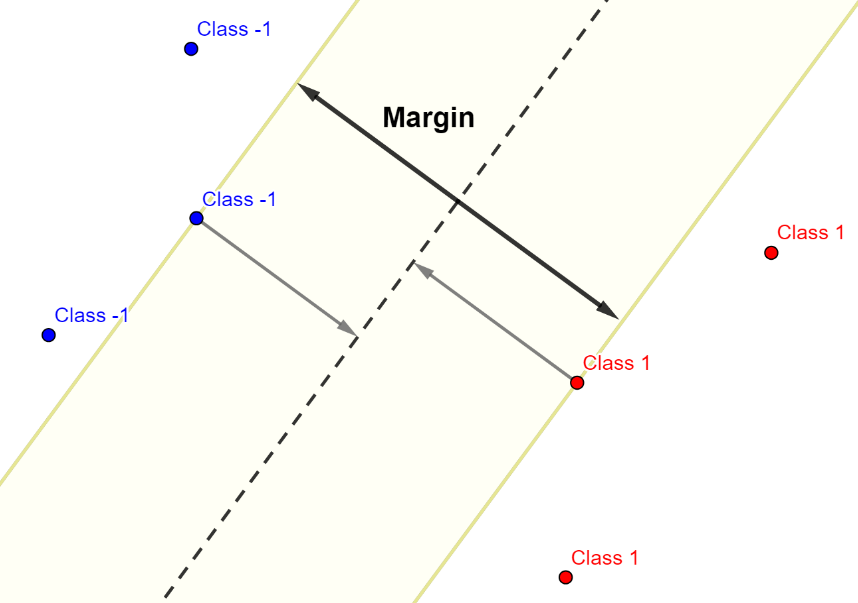
\includegraphics[width=0.7\textwidth]{SVM.png}
\captionof{figure}{Figure showing a margin (black line) between two classes of data. The variable M is shown by the grey lines.}

\end{center}

The variable M (shown as the grey lines in figure 1) is $\frac{1}{2}$ the margin distance and is the measurement of the closest point to the boundary line. The SVM algorithm finds the hyperplane that gives the maximal margin. The margin $M$ is maximised subject to the contraint
\begin{equation}
\begin{gathered}
y_i(x_i^T \beta+\beta_0)\geq M,\text{ } \forall i
\end{gathered}
\end{equation}

where $y_i$ is the target variable for a single data point $i$, formally $y_i \in \{-1, 1\}$. $\beta$ and $\beta_0$ are the coefficients of the hyperplane. In the case where the data is not linearly separable, some points are allowed to be on the wrong side of the margin. These points are then given a slack variable $\varepsilon_i$ measured as the distance inside the margin, and a new constraint is formulated:

\begin{equation}
\begin{gathered}
y_i(x_i^T \beta+\beta_0)\geq M(1-\varepsilon_i),\text{ } \forall i
\\
\sum_{i=1}^m\varepsilon_i = \text{constant}
\end{gathered}
\end{equation}

Depending on the dimensionality of the vector space of the data, and the type of “kernel” used, the geometry of the decision boundary varies. For a linear kernel the decision boundary will be a hyperplane, in 2D this is a straight line. 

The kernel (or kernel trick) describes the type of function used to create a transformation to form another dimension. The kernel trick is used to find non-linear boundaries by using a transformation to find a hyperplane in a new feature space. A good example of how the kernel trick works would be using a tranformation (on a 2D feature space) of the form $z=x^2+y^2$ to classify a circular decision boundary centered at 0. A 2-plane could then be found to be parallel to the $xy$-plane and would translate as a circular decision boundary.

\subsection{Neural Network}

A neural network is a machine learning technique that can be used for classifying data. The theory of computational neural networks was originally formulated in 1943 [McCulloch, Warren; Walter Pitts (1943). "A Logical Calculus of Ideas Immanent in Nervous Activity], however, due to the computational power needed, models were not commonly used until later on in the 20th century.  
\newline
\newline
Neural networks are constructed with layers of nodes with directed links between nodes in subsequent layers as seen in Figure 2. the first layer has a node for each input dimension or feature, whereas the last layer has a node for each possible output class or label. Between the first and last layers you can have hidden layers, with the number of layers and nodes in each layer being varied depending on the complexity of the model. Every layer excluding the output layer will have a bias node that will always be active (i.e. have a value of 1). Each node from the input layer is connect to all the nodes in the subsequent layer with a forward directed and weighted link. This repeats in the same manner to the final output layer. 

\begin{center}
\includegraphics[width=0.7\textwidth]{NN.png}
\captionof{figure}{Figure showing a simple neural network. The network contains two input nodes, one hidden layer containing a bias node and two other hidden layer nodes, and an output layer with two output nodes.}

\end{center}

To compute the activation $z$ of a node $j$ in layer $l$, the input nodes are multiplied by their relative weights and all summed
\begin{equation}
z^{(l)}_j = \sum_{i=1}^N \theta_i a^{(l-1)}_i
\end{equation}

where $N$ is the number of nodes that have links to node $j$ in layer $l$. The value of this sum is then inputted into an “activation function” that will return a value between 0 and 1. One example of an activation function commonly used is the sigmoid function, 

\begin{equation}
h(x)=\frac{1}{1+e^{-x}}
\end{equation}

To train a neural network, the weights are randomly initialised and a training sample is inputted at the first layer of nodes. The values are then fed-forward through the network to give a reading at each output node between 0 and 1, which can be heuristically interpreted in a trained model as the probability that the input is in a given class. 
\newline

At this point, the outputted values are compared to the data points given layer and the “error” of the predicted output is fed into a cost function. Using the cost value, the cost is propagated backwards through the network.  The weights are adjusted by using an optimization method, for example, gradient descent to minimise the cost as a function of the weights.

\subsection{Decision Tree}

A decision tree classifier works by using simple decision rules to identify the class of some inputted data. The feature space is partitioned repeatedly through these decision rules until the classes are grouped together. 

\begin{figure}[h]
    \centering
    \subfloat[The decision boundary produced by the decision tree graph (b)]{{\includegraphics[width=7cm]{DT.png} }}%
    \qquad
    \subfloat[The decision tree graph for inputs $x$ and $y$]{{\includegraphics[width=7cm]{DT2.png} }}%
    \caption{Figure showing the decision tree graph (b) and respective boundary (a).}%
    \label{fig:example}%
\end{figure}

The rules used to partition the space are chosen by computing the Gini impurity, which is calculated for a set of points with $J$ classes by
\begin{equation}
I_{Gini}(p, J)=1-\sum_{i=1}^Jp_i^2
\end{equation}

where $p_i$ is the fraction of items in class $i$. Gini inpurity is a measure of how mixed a subset of elements of certain classes are. To choose a rule, consider a parent set of $N$ points containing $J$ classes, and a rule that produces two child branches containing $J_0$ classes with $N_0$ data points, and $J_1$ classes with $N_1$ data points. We then measure the information gain $IG$ by looking at the parent Gini impurity, and the Gini impurity of the two child branches, and take the weighted mean

\begin{equation}
IG= N\cdot I_{Gini}(p, J) - (N_0\cdot I_{Gini}(p, J_0) + N_1\cdot I_{Gini}(p, J_1))
\end{equation}

Information gain is then measured for all possible splits, and the split that gives the highest information gain is chosen. This process is then recursively made until either a chosen $max\ depth$ is reached or all training data has been seperated.  

\newpage
\section{Optimization}

When trying to find a 2D projection of the data that produces a maximum accuracy reading, it is generally not efficient to use the Grand Tour algorithm. Instead, new rotation matrices should be constructed without the use of the Grand Tour algorithm. This is because the Grand Tour's purpose is to give a set of rotation matrices that can be combined to create a "smooth" animation that returns projections of the data from as many angles as possible. By constructing rotation matrices without the constraints of the Grand Tour, the time to find local and global maxima is decreased.

\subsection{Mathematical Construction}

In an $n$-dimensional feature space, all $n\times n$ rotation matrices will need to be elements of the special orthogonal group $SO(n)$. Therefore, new rotation matrices that are created will need a determinant of +1. This requirement puts constraints on the elements in the matrices:
\begin{equation}
\sum_{k}A_{ik}A_{jk} = \delta_{ij}
\end{equation}

where $\bm{A}$ represents the rotation matrix and $\delta_{ij}$ is the Kronecker delta. Consider the transformation equation given by equation (2), given that the projection wanted is 2D, only two rows of the rotation matrix need to be quantified. To simplify the probem the following vectors are used: 
\begin{align}
\bm{a}_1 = \begin{bmatrix}
           A_{11} \\
           A_{12} \\
           \vdots \\
           A_{1n}
           \end{bmatrix} 
           && 
\bm{a}_2 = \begin{bmatrix}
           A_{21} \\
           A_{22} \\
           \vdots \\
           A_{2n}
           \end{bmatrix}
\end{align} 

The constraint given by equation (13) can now be written as
\begin{equation}
\begin{split}
\bm{a}_1 \cdot \bm{a}_1 = 1
\\
\bm{a}_2 \cdot \bm{a}_2 = 1
\\
\bm{a}_1 \cdot \bm{a}_2 = 0
\end{split}
\end{equation}

In the vector space $\mathbb{R}^n$, $\bm{a}_1$ and $\bm{a}_2$ can be considered as vectors pointing to the edge of an $n$-sphere, but with the added constraint that they are orthogonal to each other. 
\begin{center}
\includegraphics[width=0.7\textwidth]{OrthogV.png}
\captionof{figure}{Figure showing the $n$=3 case with a sphere. The second horizontal vector can point anywhere on the dotted "equator" line to satisfy the orthogonality condition.}

\end{center}

Due to the vectors being contained on a $n$-sphere, it is natural to transform the elements of the vectors into $n$-dimensional spherical polar coordinates. Now there are new parameters for each angle used in the coordinate transformation.
\newline

\newpage
\section{Results}

\newpage
\section{Conclusion}

Using the grand tour for data mining has some interesting properties. Some insight into dimensionality reduction can be made by finding the projections that maximise the various machine learning algorithms. Looking at the relevant rotation matrices, how much of each feature or dimension appears in the new convoluted basis vectors gives insight to which features are important in distinguishing for a certain class.
\newline
\newline
One suggestion was to look into if the Hilbert curve could be used to look at the data from many different unique projections, as it uniformly covers the space. This wasn’t pursued as there is a problem in defining the projection. In 3D, a vector from a Hilbert curve node to the centre of the data uniquely defines a plane. This is because the vector can be used to take away one dimension and use 2 orthogonal unit vectors to create a basis for a subspace. However, when the dimensionality exceeds 3 there is a problem with this method. In a 4D feature space, 2 unique vectors are needed to define a unique plane. 
\newline
\newline
Something that would be interesting to investigate further is to see if a new unsupervised learning clustering algorithm could be developed to group data into classes. By looking at how much each data point moves relative to another data point in the tour (travel matrix), could this give insight to classification groupings? After looking at the matrix colourmap of this variable, three rectangular shaped structures can be seen in the ordered data. By using network community detection algorithms or some other clustering analysis, would this method work, and more importantly, how would it compare to current unsupervised learning algorithms as the travel matrix is somewhat similar to the distance between points in the feature space.

\end{document}
